\documentclass[a4paper,10pt]{article}
\usepackage[utf8]{inputenc}
\usepackage{polski}
\usepackage{amsthm}
\usepackage{amsmath}
\usepackage{amsfonts}
\usepackage[shortlabels]{enumitem}
\usepackage{amssymb}
\usepackage{xifthen}
\usepackage[top=2.5cm, bottom=2.5cm, left=3.5cm, right=2.5cm]{geometry}

\newtheorem{thm}{Twierdzenie}
\newtheorem{prop}[thm]{Stwierdzenie}
\newtheorem{df}[thm]{Definicja}
\newtheorem{note}[thm]{Spostrzeżenie}
\newtheorem{ex}[thm]{Przykład}
\newtheorem{cor}[thm]{Wniosek}
\newtheorem{lem}[thm]{Lemat}
\newtheorem{fact}[thm]{Fakt}

% \cl[X]{A} or \cl{A}
\newcommand{\cl}[2][]{%
\ifthenelse{\isempty{#1}}{\overline{#2}}{\overline{#2}^{#1}}%
}
\newcommand{\id}{\operatorname{id}}
\newcommand{\im}{\operatorname{im}}
\newcommand{\wght}{\operatorname{wght}}
\newcommand{\card}{\operatorname{card}}
\let\emptyset\varnothing % better emptyset character
\newcommand{\Ni}{{\mathbb{N}_1}}
\newcommand{\bd}{\partial} % boundary
\newcommand{\dom}{\operatorname{dom}}

% set couter like: section.couter
\numberwithin{thm}{section}
\numberwithin{equation}{section}

% use better calligraphic font (should've done find'n'replace)
\usepackage{mathrsfs}
\renewcommand{\mathcal}{\mathscr}

%opening
\title{}
\author{}

\begin{document}
  \section{Gdzie jesteśmy, szkic}
Niech $(X, d)$ będzie przestrzenią liniowo-metryczną z metryką ograniczoną przez $1$, $Y := \Pi_{i=1}^{\infty} X_i$, gdzie $X_i := X$. Obiektem naszego zainteresowania jest $Y$ z topologią produktową.

Oznaczenia:
\begin{itemize}
  \item $d_n(x, y) := \sum_{i=1}^n \frac{1}{2^i} d(x_i, y_i)$
  \item $d := d_\infty$
  \item $\rho(x, A) := \inf_{y \in A} \rho(x, y)$, gdzie $\rho$ metryka
  \item $y \in Y$, to $y = (y_i)_{i=1}^\infty$
  \item $s_n: Y \ni y \rightarrow (y_1, \ldots, y_n) \in \Pi_{i=1}^{n} X_i$
  \item utalmy punkt $x_0 \in X$. Niech $\star_n := (x_0)_{i=n+1}^\infty$
  \item będziemy utożsamiać zbiory homeomorficzne. W szczególności $Y$ i $\Pi_{i=j}^\infty$ dla dowolnego $j$.
\end{itemize}

\begin{note}[fakty topologiczne]
\begin{itemize}
  \item $\cl{A \times B} = \cl A \times \cl B$
  \item jednorodność $Y$, tzn. $Y = \Pi_{i=1}^n X \times \Pi{i=n+1}^\infty X$ z topologią produktową
  \item $\partial(A \cup B) \subset \partial A \cup \partial B$
\end{itemize}
\end{note}

  \section{Wybrane własności przestrzeni topologicznych i metrycznych}
 
\begin{df}
  Wagą przestrzeni topologicznej $M$ nazwiemy najmniejszą liczbę kardynalną $\kappa$ taką, że istnieje baza $M$ mocy $\kappa$. Piszemy wówczas $\wght M = \kappa$.
\end{df}
 
\begin{lem} \label{lem:base-small}
  Niech $M$ będzie przestrzenią topologiczną o własności $\wght M \geq \aleph_0$. Niech $\mathcal B$ będzie bazą $M$. Wówczas z $\mathcal B$ można wybrać podzbiór $\mathcal B_0$ o mocy nie większej niż waga przestrzeni, tj.:
  \[
    \card \mathcal B_0 \leq \wght M,
  \]
  który jest również bazą.
  \begin{proof}
    Niech $\mathcal D$ będzie bazą $M$ o mocy równej $\wght M$. Niech $D_0 \in \mathcal D$. Wówczas istnieje $\mathcal B_{D_0} \subset \mathcal B$, który sumuje się do $D_0$, tzn. $\bigcup \mathcal B_{D_0} = D_0$. Niech $B \in \mathcal B_{D_0}$. Ten zbiór, z kolei, sumuje się z pewnej podrodziny $\mathcal D_B$ bazy $\mathcal D$. Ale $\card\mathcal D = \wght M$, więc dla $\mathcal D_0 := \{D\ |\ D \in \mathcal D_B, B \in \mathcal B_{D_0}\}$ mamy $\card\mathcal D_0 \leq \wght M$. Dla każdego $D \in \mathcal D_0$ oznaczmy poprzez $B_D$ dowolny nadziór $D$ wpadający w $\mathcal B_{D_0}$. Wówczas $\mathcal G_{D_0} := \{B_D\ |\ D \in \mathcal D_0\}$ jest podzbiorem $\mathcal B$ mocy nie większej niż $\wght M$, który sumuje się do $D_0$.
    
    Niech
    \[
      \mathcal B_0 := \bigcup_{D_0 \in \mathcal D} \mathcal G_{D_0}
    \]
    Zbiór $\mathcal B_0$ podzbiorem $\mathcal B$ mocy nie większej niż $\wght M \cdot \wght M = \wght M$. Co więcej, jeśli $U$ jest zbiorem otwartym, to możemy go wysumować ze zbiorów bazy $\mathcal D$. Ale każdy ze zbiorów $D \in \mathcal{D}$, możemy wysumować z rodziny $\mathcal G_D \subset \mathcal B_0$. W konsekwencji zbiór $U$ daje się wysumować ze zbiorów rodziny $\mathcal B_0$, a więc $\mathcal B_0$ jest szukaną bazą.
  \end{proof}
\end{lem}
 
\begin{fact}
  Powyższy lemat zachodzi również w przypadku $\wght M < \aleph_0$.
  \begin{proof}(szkic)
    Jeśli przestrzeń $M$ ma skończoną bazę, to sama topologia jest skończona, ponieważ każdy zbiór sumuje się ze zbiorów z bazy. Będziemy konstruować bazę minimalną $\mathcal D$. Weźmy zbiory minimalne w tej topologii względem relacji porządku. Takie zbiory muszą należeć do każdej bazy. Następnie usuńmy z topologii wszystkie zbiory, które dają się wysumować ze zbiorów minimalnych. Procedurę kontynuujemy, tzn. z pozostałych zbiorów bierzemy zbiory minimalne według relacji inkluzji - one znowuż muszą należeć do każdej bazy, bo nie dają się wysumować jako nic innego. Wszystkie sumy zbiorów minimalnych usuwamy.
    
    Powyższa procedura zakończy się w skończenie wielu krokach. Z konstrukcji wynika, że ogół zbiorów minimalnych we wszystkich turach stanowi bazę minimalną oraz, że w dowolnej bazie zawarta jest owa baza minimalna. Dlatego też z $\mathcal B$ można wybrać $\mathcal B_0$ o żądanej własności.
  \end{proof}
\end{fact}
 
\begin{df}
  Łańcuchem w zbiorze $M$ nazwiemy uporządkowaną rodzinę $(U_0, \ldots, U_n)$ podzbiorów zbioru $M$ taką, że:
  \[
    \forall i \in n: U_i \cap U_{i+1} \neq \emptyset
  \]
  Zbiory $U_i$ będziemy nazywać ogniwami.
\end{df}
 
\begin{df}
  Niech $M$ będzie przestrzenią toplogiczną, a $\mathcal B$ ustaloną rodziną podzbiorów $M$. Powiemy, że przestrzeń $M$ jest $\mathcal B$-łańcuchowo spójna, jeśli każde dwa punkty $x,y \in M$ można połączyć łańcuchem $(U_0, \ldots, U_n)$ w $\mathcal B$, tj. $x \in U_0$ i $y \in U_n$, a $U_i \in \mathcal B\ \forall i \in n+1$.
\end{df}
 
\begin{lem} \label{lem:chain-connected}
  Niech $M$ będzie spójną przestrzenią topologiczną, a $\mathcal B$ bazą $M$. Wówczas $M$ jest $\mathcal B$-łańcuchowo spójna.
  \begin{proof}
    Dla ułatwienia będziemy mówić łańcuch zamiast $\mathcal B$-łańcuch.
    Jeśli $M = \emptyset$, to lemat jest prawdziwy. Niech $m_0 \in M$. Niech
    \[
      A := \{m \in M\ |\ \mbox{istnieje łańcuch od $m_0$ do $m$}\}
    \]
    Niech $m \in A$.
    Wówczas istnieje łańcuch $(U_0, \ldots, U_n)$ od $m_0$ do $m$.
    Zatem każdy punkt $m' \in U_n$ jest połączony tym samym łańcuchem $(U_0, \ldots, U_n)$ z $m_0$.
    
    \begin{figure}[h!]
      \centering
      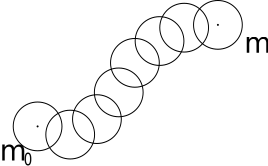
\includegraphics[scale=.5]{img/chain.pdf}
      \caption{Łańcuch od $m_0$ do $m$}
    \end{figure}
    
    Niech $m \in M\setminus A$.
    Weźmy otoczenie $U\in\mathcal B$ punktu $m$. Niech $m'\in U$ i przypuścmy, że $m'\in A$. Zatem istnieje łańcuch $(U_0, \ldots, U_n)$ łączący $m_0$ i $m'$. Ale wtedy $(U_0, \ldots, U_n, U)$ jest łańcuchem łączącym $m_0$ z $m$, czyli $m\in A$, sprzeczność. Zatem $m'\in M\setminus A$.
    
    $A$ jest więc niepustym, bo $m_0 \in A$, zbiorem otwarto-domkniętym. Ze spójności $M$ mamy $A = M$, a więc $M$ jest łańcuchowo spójne.
  \end{proof}
\end{lem}
 
\begin{df}
  Niech $Y$ będzie przestrzenią toplogiczną. Rozmaitością topologiczną modelowaną na $Y$ nazwiemy przestrzeń topologiczną parazwartą $M$ taką, że każdy punkt ma otoczenie homeomorficzne ze zbiorem otwartym w $Y$.
\end{df}
 
\begin{df}
  Atlasem na rozmaitości $M$ nazwiemy rodzinę homeomorfizmów $\{f_c : M \supset U_c \to V_c \subset Y\}_{c \in C}$ pomiędzy zbiorami otwartymi w $M$ i $Y$ -- zwanych również mapami -- taką, że $\bigcup_{c \in C} U_c = M$.
\end{df}
 
\begin{fact} \label{fact:local-metrizability}
  Jeśli $Y$ jest przestrzenią metryczną, to rozmaitość topologiczna $M$ jest również przestrzenią metryczną.
  \begin{proof}(szkic)
    $M$ jest przestrzenią lokalnie metryzowalną, jako przestrzeń lokalnie homeomorficzna z przestrzenią metryzowalną. Z definicji jest też przestrzenią parazwartą. Metryzowalność wynika z twierdzenia o metryzowalności Michaela. [patrz \ref{reference-needed}]
  \end{proof}
\end{fact}
 
\begin{thm}(Twierdzenie A. H. Stone'a)
  \label{thm:stone}
  W dowolne pokrycie otwarte przestrzeni metrycznej można wpisać pokrycie jednocześnie lokalnie skończone i $\sigma$-dyskretne.
  \begin{proof}
    Klasyczny dowód można znaleźć w \cite{ENG}.
  \end{proof}
\end{thm}
 
\begin{cor}
  Niech $Y$ będzie przestrzeią metryczną. Wówczas założenie parazwartości rozmaitości $M$ modelowanej na $Y$ jest równoważne założeniu metryzowalności.
  \begin{proof}
    Z faktu \ref{fact:local-metrizability} mamy, że parazwartość rozmaitości daje jej metryzowalność. Z twierdzenia \ref{thm:stone} wynika, że metryzowalność daje parazwartość.
  \end{proof}
\end{cor}
 
\begin{lem} \label{lem:cl-refinement}
  Niech $M$ będzie parazwartą przestrzenią topologiczną. Wówczas dla każdego pokrycia otwartego $(U_t)_{t \in T}$ przestrzeni $M$ istnieje pokrycie otwarte $(U_t')_{t \in T}$ takie, że $\cl{U_t'}\ \subset U_t\ \forall t \in T$.
  \begin{proof}
    Dowód można znaleźć w \cite{ENG}.
  \end{proof}
\end{lem}
 
\begin{df}
  Pokrycie $(U_t)_{t \in T}$ przestrzeni topologicznej nazwiemy $\star$-skończone, gdy gwiazda każdego elementu tego pokrycia składa się ze skończenie wielu elementów, tj.:
  \[
    \forall t_0 \in T: \card\{t \in T\ |\ U_t \cap U_{t_0} \neq \emptyset\} < \aleph_0
  \]
\end{df}
 
\begin{lem} \label{lem:star-finite}
  Niech $M$ będzie parazwartą przestrzenią topologiczną. Wówczas dla każdego przeliczalnego pokrycia otwartego $M$ istnieje przeliczalne pokrycie otwarte wpisane, $\star$-skończone.
  \begin{proof}
    Dowód można znaleźć w \cite{bp}.
  \end{proof}
\end{lem}
 
\begin{df}
  Powiemy, że rodzina $(U_n)_{n\in\Ni}$ jest uporządkowana w sposób łancuchowo skończony, jeśli nie istnieje nieskończony łańcuch elementów tej rodziny indeksowany silnie rosnącym ciągiem, tzn. nie istnieje $(i_n)_{n\in\Ni}$:
  \[
    i_n < i_{n+1} \wedge U_{i_n} \cap U_{i_{n+1}} \neq \emptyset\ \forall n\in\Ni
  \]
\end{df}
 
\begin{lem} \label{lem:chain-finite-order}
  Każda przeliczalna $\star$-skończona rodzina posiada łańcuchowo skończony porządek.
  \begin{proof}
    Dowód można znaleźć w \cite{bp}.
  \end{proof}
\end{lem}
  \section{Wybrane własności przestrzeni liniowo-metrycznych}

\begin{df}
  Niech $(Y, d)$ będzie przestrzenią liniowo-metryczną. Metrykę $d$ nazwiemy niezmienniczą, gdy zachodzi warunek:
  \[d(x+a, y+a) = d(x,y)\ \forall x, y, a \in Y\] 
\end{df}


\begin{fact}
  Na dowolnej przestrzeni liniowo-metrycznej $Y$ z metryką $d$ można wprowadzić metrykę niezmienniczą.
  
  \begin{proof}(szkic) Przestrzeń liniowo-metryczna z operacją $+$ stanowi grupę topologiczną z topologią zadaną przez metrykę, a więc spełniającą pierwszy aksjomat przeliczalności oraz własność $T_2$. Z twierdzenia Birkhoffa-Kakutaniego \cite{bir}, \cite{kak} istnieje więc na niej metryką lewostronnie niezmiennicza.
  \end{proof}
\end{fact}

\begin{note}
  Niech $(Y, d)$ przestrzeń liniowo-metryczna z metryką niezmienniczą. Wówczas metryka $\rho := \min(d, 1)$ jest ograniczoną, niezmienniczą metryką równoważną.
  \begin{proof}
    Równoważność wynika z równości małych kul, tzn. $\forall n \in \mathbb{N}_1: B_\rho(0, \frac{1}{n}) = B_d(0, \frac{1}{n})$. Metryka $\rho$ jest oczywiście ograniczona przez 1. Z równości:
    \[
      \rho(x+a, y+a) = \min(d(x+a, y+a), 1) = \min(d(x,y), 1) = \rho(x,y)
    \]
    wnioskujemy, że $\rho$ jest metryką niezmienniczą.
  \end{proof}
\end{note}


Z uwagi na powyższy fakt na przestrzeniach liniowo-metrycznych będziemy rozważali tylko ograniczone przez $1$ metryki niezmiennicze.

\begin{df}
  Niech $(Y, d)$ będzie przestrzenią liniowo-metryczną. Metrykę $d$ nazwiemy rosnącą po promieniach, gdy:
  \[d(t_1 x, 0) < d(t_2 x, 0)\ \forall 0 \leq t_1 < t_2\ \forall x \neq 0\]
  
  Gdy powyższa nierówność jest prawdziwa w wersji słabej ($\leq$) metrykę taką nazwiemy słabo rosnącą po promieniach.
\end{df}

\begin{lem}
  Aby metryka $d$ była rosnąca po promieniach wystarczy aby warunek $d(t_1 x, 0) < d(t_2 x, 0)$ zachodził dla liczb wymiernych $0 \leq t_1 < t_2$ i $x \neq 0$.
  
  \begin{proof}
    Niech $0 \leq a < b$ będą liczbami rzeczywistymi.
    Wówczas istnieją silnie monotoniczne ciągi $(a_n)_{n=1}^\infty$ oraz $(b_n)_{n=1}^\infty$ liczb wymiernych takie, że $a_n \downarrow a$ i $b_n \uparrow b$ oraz $a_1 < b_1$. Zatem $\forall n > 1$:
    \[d(a_n x, 0) < d(a_1 x, 0) < d(b_1 x, 0) < d(b_n x, 0)\]
    
    Co po przejściu granicznym daje:
    \[d(a x, 0) \leq d(a_1 x, 0) < d(b_1 x, 0) \leq d(b x, 0)\]
    
    Zatem $d(ax, 0) < d(bx, 0)$. 
  \end{proof}
\end{lem}


\begin{thm}[Eidelheit-Mazur] \label{thm:eidelheit-mazur} \cite{em}
  Niech $(Y, d)$ przestrzeń liniowo-metryczna. Wówczas istnieje ograniczona przez $1$, niezmiennicza metryka $\rho$ równoważna $d$ rosnąca po promieniach.
  \begin{proof}
    Określamy dla $w > 0$ metrykę $\rho_w(x, y) := \sup_{0 \leq t \leq w} d(tx, ty)$. $\rho_w$ jest metryką, jako skończone supremum metryk ograniczonych przez $1$. Z niezmienniczości $d$ wynika niezmieniczość $\rho_w$. Co więcej, $\rho_w$ jest metryką równoważną $d$.
    
    Istotnie:
    \begin{align*}
      \rho_w(x_n, x) \to 0 &\implies 0 \leq d(w x_n, wx) \leq \rho_w(x_n,x)  \to 0 \\
      &\implies d(wx_n, wx) \to 0 \\
      &\implies d(x_n, x) \to 0
    \end{align*}
    gdzie ostatnia implikacja wynika z ciągłości mnożenia (mnożymy przez $w^{-1}$).
    
    Z drugiej strony, niech $d(x_n, x) \to 0$ oraz $\varepsilon > 0$. Zdefiniujmy odwzorowanie:
    \[m: [0,w] \times Y \ni (t,x) \to d(tx, 0) \in [0,\infty)\]
    
    Z ciągłości $m$ wynika, że dla każdego $t$ istnieje $V_t$ otoczenie $t$ oraz $U_t$ otoczenie $0$ w $Y$ takie, że $m(s, y) < \varepsilon$ o ile tylko $s \in V_t$ i $y \in U_t$.
    
    Ze zwartości odcinak $[0,w]$ wybieramy z pokrycia $\{V_t\}_{t \in [0,w]}$ skończone podpokrycie $(V_{t_i})_{i=1}^{k}$.
    
    Biorąc $U := \bigcap_{i=1}^k U_{t_i}$ otrzymujemy otwarte otoczenie $0$ o własności:
    \[\mbox{Jeśli }t \in [0,w]\mbox{ i }x \in U,\mbox{ to } m(t,x) = d(tx, 0) < \varepsilon\]
    
    Ustalmy $n_0$ tak, aby dla każdego $n \geq n_0$ było $x_n - x \in U$. Ale wtedy:
    \[\rho_w(x_n, x) = \rho_w(x_n - x, 0) = \sup_{0 \leq t \leq w} d(t(x_n - x), 0) \leq \varepsilon\]
    
    A więc $\rho_w(x_n, x) \to 0$, co dowodzi równoważności $\rho_w$ i $d$.
    
    Zauważmy jeszcze, że $\rho_w$ jest metryką słabo rosnącą po promieniach. Rzeczywiście, niech $0 \leq t_1 < t_2$, $x \in Y$. Mamy:
    \[\rho_w(t_1 x, 0) = \sup_{0 \leq t \leq w} d(t \cdot t_1 x, 0) \leq \sup_{0 \leq t \leq w} d(t \cdot t_2 x, 0) = \rho_w(t_2 x, 0)\]
    
    Ułóżmy wszystkie liczby wymierne dodatnie w ciąg $(w_i)_{i=1}^\infty$. Definiujemy wynikową metrykę jako:
    \[\rho(x, y) := \sum_{i=1}^\infty \frac{1}{2^i} \rho_{w_i}(x, y)\]
    
    Zbieżność powyższego szeregu wynika z ograniczoności metryk $\rho_w$ przez $1$, co więcej $\rho(x,y) \leq 1$. Z niezmienniczości metryk $\rho_w$ wynika niezmienniczość $\rho$. Ponadto metryka $\rho$ jest równoważna metryce $d$.
    
    Istotnie, metryka $\rho$ jest większa niż $\frac{1}{2} \rho_{w_1}$, która jest równoważna metryce $d$, a więc $\rho(x_n, x) \to 0$ pociąga $d(x_n, x) \to 0$.
    
    Z drugiej strony, niech $d(x_n, x) \to 0$ i $\varepsilon > 0$. Z równoważności $d$ i $\rho_w$ mamy $\rho_w(x_n, x) \to 0$.
    
    Ustalmy $k \in \mathbb{N}_1$ takie, że $\sum_{i=k+1}^\infty \frac{1}{2^i} < \frac{\varepsilon}{2}$.
    Ustalmy teraz $n_0 \in \mathbb{N}_1$ takie, że:
    \[\forall i \in [1,k]\ \forall n > n_0: \frac{1}{2^i} \rho_{w_i}(x_n, x) \leq \frac{\varepsilon}{2k}\]
    
    Wówczas $\forall n > n_0$:
    \[\rho(x_n, x) \leq \sum_{i=1}^k \frac{1}{2^i} \rho_{w_i}(x_n, x) + \sum_{i=k+1}^\infty \frac{1}{2^i} \leq k \cdot \frac{\varepsilon}{2k} + \frac{\varepsilon}{2} = \varepsilon\]
    a więc $\rho(x_n, x) \to 0$
    
    Pokażemy teraz, że metryka $\rho$ jest rosnąca po promieniach. Ustalmy $0 \leq t_1 < t_2$ oraz $x \in Y$. Z poprzedniego lematu wiemy, że wystarczy rozważyć jedynie $t_1, t_2 \in \mathbb{Q}$. Ze słabego wzrostu po promieniach metryk $\rho_{w_i}$ wynika słaby wzrost po promieniach metryki $\rho$. Wystarczy więc wykazać, że dla pewnego $i$ zachodzi $\rho_{w_i}(t_1 x, 0) < \rho_{w_i}(t_2 x, 0)$. Przypuśćmy dla dowodu niewprost, że $\forall i: \rho_{w_i}(t_1 x, 0) = \rho_{w_i}(t_2 x, 0)$. Weźmy ciąg malejący do zera ciąg liczb wymiernych: $(t_1^i t_2^{-i})_{i=0}^\infty$ i przyjrzyjmy się metrykom $\rho_w$ związanym z kolejnymi wyrazami tego ciągu. Najpierw zanotujmy:
    \begin{align*}
      \rho_{t_1^i t_2^{-i}}(t_1 x, 0) = \sup_{0 \leq t \leq t_1^i t_2^{-i}} d(t \cdot t_1 x, 0) =
      \sup_{0 \leq t \leq t_1^{i+1} t_2^{-(i+1)}} d(t \cdot t_2 x, 0) = \rho_{t_1^{i+1} t_2^{-(i+1)}}(t_2 x, 0)
    \end{align*}
    Skąd otrzymujemy ciąg równości:
    \begin{align*}
      \rho_1(t_2 x, 0) &= \rho_1(t_1 x, 0) = \\
      \rho_{t_1 t_2^{-1}}(t_2 x, 0) &= \rho_{t_1 t_2^{-1}}(t_1 x, 0) = \\
      \rho_{t_1^2 t_2^{-2}}(t_2 x, 0) &= \rho_{t_1^2 t_2^{-2}}(t_1 x, 0) = \\
      \cdots
    \end{align*}
    A więc
    \begin{align*}
      d(t_2 x, 0) \leq \sup_{0 \leq t \leq 1} d(t \cdot t_2 x, 0) &= \rho_1(t_2 x, 0) \\
      &= \rho_{t_1^i t_2^{-i}}(t_1 x, 0) = \sup_{0 \leq t \leq t_1^i t_2^{-i}} d(t \cdot t_1 x, 0)
    \end{align*}
    Z równoważności metryki $d$ i $\rho_{t_1}$ wynika, że skoro $t_1^i t_2^{-i} \to 0$ --- a więc i $d(t_1^i t_2^{-i} x, 0) \to 0$ --- to:
    \[
      \sup_{0 \leq t \leq t_1^i t_2^{-i}} d(t \cdot t_1 x, 0)
      = \sup_{0 \leq t \leq t_1} d(t \cdot t_1^i t_2^{-i} x, 0)
      = \rho_{t_1}(t_1^i t_2^{-i} x, 0)
    \]
    również dąży do zera. Zatem $d(t_2 x, 0) = 0$, co w konsekwencji daje $x = 0$. Zatem jedynym przypadkiem, gdy nie zachodzi wzrost po promieniach jest $x = 0$, zatem $\rho$ jest metryką rosnącą po promieniach.
  \end{proof}
\end{thm}

\begin{lem} \label{lem:ball-homeomorphism}
  Niech $Y$ będzie przestrzenią liniowo-metryczną. Wówczas przestrzeń $Y$ z metryką rosnącą po promieniach $d$ spełnia warunek: dla każdego $\varepsilon > 0$ kula $U_\varepsilon := B_d(0, \varepsilon)$ jest homeomorficzna z $Y$.
  
  \begin{proof}
    Weźmy metrykę $d$ na $Y$ rosnącą po promieniach z twierdzenia Eidelheita-Mazura. Niech $0 < t_1 < t_2$. Pokażemy, że:
    \[
      \cl{t_1 U_\varepsilon} \subset t_2 U_\varepsilon
    \]
    
    Istotnie, niech $y \in \cl{t_1 U_\varepsilon}$. Wówczas istnieje ciąg $(y_n)_{n=1}^\infty \in U_\varepsilon^{\mathbb{N}_1}$ taki, że $t_1 y_n \to y$. Wynika stąd, że $d(y_n, 0) < \varepsilon$ a po przejściu granicznym $d(\frac{y}{t_1}, 0) \leq \varepsilon$. Ale z monotoniczności metryki $d$ mamy: $d(\frac{y}{t_2}, 0) < d(\frac{y}{t_1}, 0) \leq \varepsilon$ a więc $y \in t_2 U_\varepsilon$.
    
    Definiujemy odwzorowanie:
    \[
      \lambda: Y \ni y \to \inf \{t \geq 0\ |\ y \in t U_\varepsilon\} \in [0, \infty)
    \]
    
    Podobnie jak w przypadku funkcjonału Minkowskiego pokażemy, że $\lambda$ spełnia warunek:
    \[
      y \in t_0 U_\varepsilon \iff \lambda(y) < t_0
    \]
    
    Istotnie, niech $y \in t_0 U_\varepsilon$
    Wówczas z otwartości zbioru $U_\varepsilon$ i ciągłości mnożenia istnieje $t_1 < t_0$ takie, że $y \in t_1 U_\varepsilon$.
    A więc $\lambda(y) \leq t_1 < t_0$.
    Z drugiej strony, jeśli $\lambda(y) < t_0$, to z definicji infimum istnieje $t_1 < t_0$ takie, że $y \in t_1 U_\varepsilon$, ale $\cl{t_1 U_\varepsilon} \subset t_0 U_\varepsilon$, więc $y \in t_0 U_\varepsilon$.

    Wykażemy ciągłość odwzorowania $\lambda$.
    Ustalmy $y_0 \in Y$ oraz $\lambda(y_0) > \delta > 0$.
    Niech $U := (\lambda(y_0) + \delta) U_\varepsilon \setminus \cl{(\lambda(y_0)-\delta) U_\varepsilon}$.
    
    Po pierwsze zauważmy, że $y_0 \in U$.
    Istotnie, skoro $\lambda(y_0) < \lambda(y_0) + \delta$, to $y_0 \in (\lambda(y_0) + \delta) U_\varepsilon$.
    Z drugiej strony, gdyby $y_0 \in \cl{(\lambda(y_0) - \delta) U_\varepsilon} \subset (\lambda(y_0) - \frac{\delta}{2}) U_\varepsilon$, to $\lambda(y_0) < \lambda(y_0) - \frac{\delta}{2}$.
    Zatem $U$ jest otwartym otoczeniem $y_0$.
    
    Następnie zauważmy, że jeśli $y \in (\lambda(y_0) + \delta) U_\varepsilon$, to $\lambda(y) < \lambda(y_0) + \delta$ oraz jeśli $y \not\in \cl{(\lambda(y_0) - \delta) U_\varepsilon}$, to $\lambda(y) \geq \lambda(y_0) - \delta$, gdyż w przeciwnym razie $\lambda(y) < \lambda(y_0) - \delta$ a więc $y \in (\lambda(y_0) - \delta) U_\varepsilon$.
    
    Jeśli natomiast $\lambda(y_0) = 0$, wystarczy wziąć otoczenie $U := (\lambda(y_0) + \delta)U_\varepsilon$. Dla każdego $y \in U$ dostajemy wówczas: $0 \leq \lambda(y) < \lambda(y_0) + \delta$.
    
    Podsumowując: $y \in U$, to $\lambda(y_0) - \delta \leq \lambda(y) < \lambda(y_0) + \delta$, a więc z dowolności $\delta$ wykazaliśmy ciągłość $\lambda$.
    
    Warto jeszcze zaznaczyć, że $\lambda(sy) = \inf \{t \geq 0\ |\ sy \in t U_\varepsilon\} = s\inf \{t \geq 0\ |\ y \in t U_\varepsilon\} = s \lambda(y)\ \forall s \geq 0, y \in Y$.
    
    Definiujemy oczekiwany homeomorfizm jako:
    \[
      h: Y \ni y \to \frac{y}{\max\left(1, \lambda(y) + \frac{1}{2}\right)} \in U_\varepsilon
    \]
    Bezpośrednio ze wzoru wynika, że $h$ jest funkcją ciągłą. Aby sprawdzić, że jest poprawnie określona należy zbadać, czy $h(y) \in U_\varepsilon$. Sprawdzimy więc:
    
    \begin{align*}
      \lambda\left(\frac{y}{\max\left(1, \lambda(y) + \frac{1}{2}\right)}\right) =
      \frac{\lambda(y)}{\max\left(1, \lambda(y) + \frac{1}{2}\right)} \leq
      \frac{\lambda(y)}{\lambda(y) + \frac{1}{2}} < 1
    \end{align*}
    A więc $h(y) \in 1 U_\varepsilon = U_\varepsilon$.
    
    Funkcją odwrotną do $h$ jest następująca funkcja ciągła:
    \[
      g: U_\varepsilon \ni z \to \frac{z}{2(1-\max(\lambda(z), \frac{1}{2}))} \in Y
    \]
    Istotnie. Funkcja $g$ jest poprawnie określona, bo dla $z\in U_\varepsilon$ mamy $\lambda(z) < 1$. Pokażemy teraz, że $g(h(y)) = y$. Jeśli $\lambda(y) \leq \frac{1}{2}$, to $h(y) = y$ oraz $g(y) = y$. Zatem $g(h(y)) = y$. Jeśli natomiast $\lambda(y) > \frac{1}{2}$, to $h(y) = \frac{y}{\lambda(y)+\frac{1}{2}}$. Wówczas jednak $\lambda(h(y)) = \frac{\lambda(y)}{\lambda(y)+\frac{1}{2}} > \frac{1}{2}$, ponieważ dla $s \geq 0$:
    \begin{align*}
      s > \frac{1}{2} \iff s > \frac{1}{2}\left(s + \frac{1}{2}\right) \iff \frac{s}{s+\frac{1}{2}} > \frac{1}{2}
    \end{align*}
    A więc:
    \begin{align*}
      g(h(y)) = g\left(\frac{y}{\lambda(y)+\frac{1}{2}}\right) &= \frac{y}{\lambda(y)+\frac{1}{2}} \cdot \frac{1}{2\left(1-\lambda\left(\frac{y}{\lambda(y)+\frac{1}{2}}\right)\right)} \\
      &= \frac{y}{\lambda(y)+\frac{1}{2}} \cdot \frac{1}{2\left(1-\frac{\lambda(y)}{\lambda(y)+\frac{1}{2}}\right)} \\
      &= \frac{y}{\lambda(y)+\frac{1}{2}} \cdot \frac{1}{2\left(\frac{\frac{1}{2}}{\lambda(y)+\frac{1}{2}}\right)} = y
    \end{align*}
    Podobnym rachunkiem łatwo sprawdzić, że $h(g(z)) = z$.
  \end{proof}
\end{lem}

W dalszym ciągu będziemy rozważali przestrzenie liniowo-metryczne z metryką niezmienniczą, ograniczoną przez $1$ i rosnącą po promieniach.

\begin{df}
  Niech $r > 0$. Podzbiór $A$ przestrzeni metrycznej $M$ nazwiemy $r$-rozstrzelonym, jeśli:
  \[
    \forall x, y \in A: d(x,y) \geq r
  \]
  Podzbiór $A$ przestrzeni metrycznej $M$ nazwiemy $r$-siecią, jeśli:
  \[
    \forall x \in M\ \exists a \in A: d(x,a) < r
  \]
\end{df}

\begin{lem} \label{lem:anti-net}
  Niech $M$ będzie przestrzenią metryczną, $r > 0$. Wówczas w $M$ istnieje maksymalny zbiór $r$-rozstrzelony. Ponadto, maksymalny zbiór $r$-rozstrzelony jest $r$-siecią.
  \begin{proof}
    Zbiór wszystkich zbiorów $r$-rozstrzelonych jest niepusty, ponieważ $\emptyset$ jest zbiorem $r$-roz\-strze\-lo\-nym, i częściowo uporządkowany przez inkluzję. Weźmy łańcuch zbiorów $r$-rozstrzelonych. Wówczas suma wszystkich elementów wszystkich zbiorów łańcucha jest również zbiorem $r$-roz\-strze\-lo\-nym. Istotnie, gdyby tak nie było, to istniałyby dwa punkty oddalone od siebie o mniej niż $r$. Ale wówczas istniałby element łańcucha zawierający oba z nich. Sprzeczność. Lemat Kuratowskiego-Zorna kończy dowód dając element maksymalny $A$.
    
    Gdyby zbiór ten nie był $r$-siecią istniałby punkt $x$ oddalony od dowolnego punktu zbioru $A$ o co najmniej $r$. Zatem zbiór $A \cup \{x\}$ byłby istotnie większym zbiorem $r$-rozstrzelonym.
  \end{proof}
\end{lem}

\begin{lem} \label{lem:balls-many}
  Niech $Y$ będzie przestrzenią liniowo-metryczną. Wówczas istnieje $A \subset Y$ o mocy $\card A \geq \wght Y$ oraz dyskretna rodzina kul $\{B(y, r_y)\}_{y \in A}$.
  
  \begin{proof}
    Gdy $Y = \{0\}$, to twierdzenie jest prawdziwe. Niech więc $Y$ będzie przestrzenią nietrywialną.
    Najpierw znajdziemy w $Y$ promień $r > 0$ oraz przeliczalną dyskretną rodzinę kul o promieniu $r$. Niech $y_0 \in Y\setminus\{0\}$. Kładziemy $r := \frac{1}{4} d(y_0,0)$. Wówczas rodzina kul: $\{B(ny_0, r)\}_{n \in \mathbb{N}_1}$ jest przeliczalna i dyskretna. Istotnie, dobrym otoczeniem punktu $y \in Y$ jest kula $B(y,r)$, ponieważ odległość dwu różnych środków $n_1 y$ i $n_2 y$, dla $n_1 < n_2$ wynosi:
    \[
      d(n_2 y_0, n_1 y_0) = d((n_2 - n_1)y_0, 0) \geq d(y_0, 0) = 4r
    \]
    Oznaczmy przez $B := B(0,r)$. Weźmy dla $n > 0$ z lematu \ref{lem:anti-net} maksymalny zbiór $\frac{r}{n}$-rozstrzelony w $B$ i oznaczmy go przez $A_n$. Zauważmy, że zbiór $\{B(y, \frac{r}{n})\ |\ y \in A_n, n \in \mathbb{N}_1\}$ jest bazą $B$. Istotnie, niech $y \in B$, weźmy $\varepsilon > 0$ takie, że $B(y,\varepsilon) \subset B$. Wówczas biorąc $n$ takie, że $2 \cdot \frac{r}{n} < \varepsilon$ znajdujemy z lematu \ref{lem:anti-net} punkt $a$ zbioru $A_n$ oddalony od $y$ o mniej niż $\frac{r}{n}$. Wówczas kula $B(a, \frac{r}{n})$ zawiera $y$ i zawiera się w $B(y,\varepsilon)$.
    
    Wynika stąd, że $\card \bigcup_{n=1}^\infty A_n \geq \wght B = \wght Y$.
    
    Wystarczy teraz każdą rodzinę kul związaną ze swoim zbiorem $\frac{r}{n}$-rozstrzelonym umieścić w osobnej kuli $B(ny_0, r)$, tzn. szukana rodzina kul wygląda następująco:
    \[
      \left\{B\left(ny_0 + y, \frac{r}{2n}\right)\ \middle|\ n \in \mathbb{N}_0, y \in A_n\right\}
    \]
    Istotnie, niech $y \in Y$. Wówczas kula $B(y,r)$ zahacza o co najwyżej jedną z kul $B(ny_0, r)$. Wystarczy więc pomniejszyć ją do kuli o promieniu mniejszym niż $\frac{r}{2n}$ aby zahaczała o co najwyżej jedną z kul wewnątrz $B(ny_0, r)$.
  \end{proof}
\end{lem}


  \section{Wybrane własności rozmaitości nieskończenie wymiarowych}

\begin{lem} \label{lem:basic-atlas}
  Niech $Y$ będzie przestrzenią liniowo-metryczną, $M$ przestrzenią topologiczną. Wówczas następujące wartunki są równoważne:
  \begin{enumerate}
   \item[(i)] każdy punkt $x \in M$ ma otoczenie homeomorficzne ze zbiorem otwartym w $Y$
   \item[(ii)] każdy punkt $x \in M$ ma otoczenie homeomorficzne z przestrzenią $Y$
   \item[(iii)] każdy punkt $x \in M$ ma bazę otoczeń homeomorficznych z $Y$
  \end{enumerate}

  \begin{proof}
    Implikacje $(iii) \implies (ii) \implies (i)$ są jasne.
    
    Pokażemy, że $(i) \implies (iii)$. Niech $x \in M$ oraz niech $f: M \supset U \to V \subset Y$ będzie mapą w otoczeniu $x$. Niech $\varepsilon_0 > 0$ będzie taki, że $B(f(x), \varepsilon_0) \subset V$. Niech $\varepsilon < \varepsilon_0$. Z lematu \ref{lem:ball-homeomorphism} istnieje homeomorfizm $g: B(f(x), \varepsilon) \to Y$, bo kula $B(0, \varepsilon)$ w przestrzeni liniowo-topologicznej jest homeomorficzna z kulą $B(f(x), \varepsilon)$. Niech $f_0$ będzie homeomorfizmem powstałym z zawężenia $f$ w obrazie do $B(f(x), \varepsilon)$ i dziedzinie do $G_\varepsilon := f^{-1}(B(f(x), \varepsilon))$. Wówczas $f_0 \circ g$ jest homeomorfizmem między $G_\varepsilon$ a $Y$.
    
    Skoro $\{B(f(x), \varepsilon)\}_{0 < \varepsilon < \varepsilon_0}$ jest bazą w punkcie $f(x)$, to $\{G_\varepsilon\}_{0 < \varepsilon < \varepsilon_0}$ jest bazą w punktcie $x$.
  \end{proof}
\end{lem}

\begin{lem}
  Niech $Y$ będzie nietrywialną przestrzenią liniowo-metryczną, a $M$ spójną rozmaitością topologiczną modelowaną na $Y$. Wówczas:
  \[
    \wght Y = \wght M
  \]
  \begin{proof}
    Niech $\mathcal U_0$ będzie pokryciem $M$ złożonym ze zbiorów homeomorficznych ze zbiorami otwartymi w $Y$. Z parazwartości wpisujemy w $\mathcal U_0$ pokrycie otwarte, lokalnie skończone $\mathcal U$.
    
    Niech $x \in M$, weźmy otoczenie $U$ punktu $x$, które przecina skończenie wiele elementów $\mathcal U$. Z lematu \ref{lem:basic-atlas} weźmy bazę otoczeń $x$ zawartą w $U$. Otrzymujemy więc rodzinę $\{U_n^x\}_{n \in \mathbb{N}_1}$ punktu $x$ o tej własności, że dla każdego $n \in \mathbb{N}_1$ mamy $\card\{U \in \mathcal U\ |\ U \cap U_n^x \neq \emptyset\} < \aleph_0$ oraz, że każdy ze zbiorów $U_n^x$ jest homeomorficzny z $Y$. Biorąc $\mathcal B := \{U_n^x\ |\ n\in\Ni, x\in M\}$ dostajemy bazę $M$.
    
    Ustalmy $U \in \mathcal U$. Wtedy $\mathcal B_U := \{B \in \mathcal B\ |\ B \subset U\}$ jest bazą $U$. Z lematu \ref{lem:base-small} wybieramy z $\mathcal B_U$ podzbiór $\mathcal D_U$, który jest bazą przestrzeni $U$ o własności:
    \[
      \card \mathcal D_U \leq \wght U
    \]
    Ale $U$ jest homeomorficzne ze zbiorem otwartym w $Y$, zatem $\wght U = \wght Y$. Nierówność $\wght U \leq \wght Y$ jest jasna, druga z nich wynika z tego, że obraz $U$ przez homeomorfizm jest zbiorem otwartym, więc zawiera w sobie jakąś kulę. A kula w $Y$ jest homeomorficzna z $Y$. Zatem $\wght Y = \wght U$.
    
    Dalej weźmy bazę $M$ postaci $\mathcal D := \bigcup_{U \in \mathcal U} \mathcal D_U$.
    
    Niech $D \in \mathcal D$. Wówczas istnieje jedynie skończenie wiele $U \in \mathcal U$ przecinających $D$, powiedzmy $U_1, \ldots, U_n$, a więc $D$ może przecinać jedynie elementy zbiorów $\mathcal D_{U_i}$, których jest w sumie co najwyżej $\aleph_0 \cdot \wght Y = \wght Y$.
    
    Ustalmy $m_0 \in M$ i weźmy wszystkie $\mathcal D$-łańcuchy zaczynające się w $m_0$. Zauważmy, że wszystkich łańcuchów zaczynających się w $m_0$ jest jedynie $\wght Y$. Istotnie, pierwsze ogniwo trzeba wybrać ze zbioru $\mathcal D_{U_1} \cup \ldots \cup \mathcal D_{U_n}$, gdzie $U_1, \ldots, U_n$ to wszystkie zbiory $\mathcal U$, które zawierają $m_0$, zatem do wyboru mamy $\wght Y$ zbiorów. Każde kolejne ogniwo musi przecinać się z poprzednim i należeć do $\mathcal D$, a takich zbiorów jest, jak już wiemy, $\wght Y$. Zatem w sumie łańcuchów zaczynających się w $m_0$ jest co najwyżej $\aleph_0 \cdot \wght Y = \wght Y$.
    
    Niech $D \in \mathcal D$, niech $x \in Y$. Z łańcuchowej spójności (\ref{lem:chain-connected}) wiemy, że $m_0$ i $x$ możemy połączyć łańcuchem $(U_1, \ldots, U_n)$. Ciąg $(U_1, \ldots, U_n, D)$ jest również łańcuchem zaczynającym się w $m_0$. Biorąc rzutowanie z rodziny wszystkich łańcuchów na ostatnie ogniwo otrzymujemy suriekcję ze zbioru mocy $\wght Y$ na $\mathcal D$, zatem $\mathcal D$ jest bazą $M$ mocy $\wght Y$.
  \end{proof}
\end{lem}

\begin{df}
  Niech $Y$ będzie przestrzenią liniowo-metryczną a $M$ $Y$-rozmaitością. Atlasem regularnym na $M$ nazwiemy atlas $\mathcal F := \{f_c: M \supset U_c \to V_c \in Y\}_{c \in C}$ taki, że każde $f: U \to V \in \mathcal F$ jest mapą regularną, tzn.:
  \begin{enumerate}[(1)]
    \item $f$ jest homeomorfizmem pomiędzy zbiorami otwartymi $U$ i $V$
    \item $f$ przedłuża się do homeomorfizmu $\cl{f}$ pomiędzy zbiorami domkniętymi $\cl U \to \cl V$
  \end{enumerate}
  Zatem $f$ jest włożeniem otwartym, a $\cl f \supset f$ jest włożeniem domkniętym.
\end{df}

\begin{lem} \label{lem:map-restriction}
  Niech $f: U \to V$ będzie mapą regularną na rozmaitości $M$ modelowanej na przestrzeni liniowo-metrycznej $Y$, niech $U_1 \subset U$ będzie zbiorem otwartym. Wówczas kładąc $V_1 := f(U_1) \subset V$ otrzymujemy $g: U_1 \to V_1 \subset f$ mapę regularną.
  \begin{proof}
    $g$ jest homeomorfizmem jako zawężenie homeomorfizmu w dziedzinie i odpowiadającym mu obrazie. Skoro $U_1$ jest zbiorem otwartym (zarówno w $U$ jak i w $M$, ponieważ $U$ jest otwarty), to $V_1$ jest zbiorem otwartym w $V$, jako obraz zbioru otwartego przez homeomorfizm, a więc i otwartym w $Y$.
    
    Co więcej:
    \[
      \cl{f}(\cl{U_1}) = \cl{f}(\cl{U_1} \cap \cl{U}) = \cl{f}(\cl[\cl{U}]{U_1}) = \cl[\cl{V}]{\cl{f}(U_1)} = \cl{\cl{f}(U_1)} \cap \cl{V} = \cl{V_1} \cap \cl{V} = \cl{V_1}
    \]
    zatem $\cl{g}$ zdefiniowane jako zawężenie $\cl{f}$ do $\cl{U_1}$ w dziedzinie i $\cl{V_1}$ w obrazie jest homeomorfizmem pomiędzy zbiorami domkniętymi, a więc $g: U_1 \to V_1$ jest mapą regularną.
  \end{proof}
\end{lem}

\begin{lem} \label{lem:map-regular}
  Niech $Y$ będzie przestrzenią liniowo-metryczną, niech $M$ będzie $Y$-rozmaitością. Dla dowolnej mapy $f: U \to V$ istnieje przeliczalna rodzina $f_n: U_n \to V_n$ map regularnych taka, że $\cl{f_n} \subset f$ oraz $\bigcup_{n=1}^\infty U_n = U$.
  \begin{proof}
    Weźmy z własności $T_6$ przestrzeni metrycznej $Y$ rodzinę zbiorów otwartych $(V_n)_{n=1}^\infty$ taką, że $\cl{V_n} \subset V_{n+1}$ i $\bigcup_{n=1}^\infty V_n = V$. Kładziemy $U_n := f^{-1}(V_n)$. Wówczas $\bigcup_{n=1}^\infty U_n = U$ oraz $\cl{U_n} = \cl{f^{-1}(V_n)} \subset f^{-1}(\cl{V_{n}}) \subset f^{-1}(V_{n+1}) = U_{n+1}$. A więc definiujemy:
    \[
      \cl{f_n}: \cl{U_n} \to \cl{V_n},\qquad \cl{f_n}(x) := f(x)
    \]
    Zauważmy, że:
    \[
      \cl{f_n}(\cl{U_n}) = f(\cl{U_n}) = f(\cl{U_n} \cap U) = f(\cl[U]{U_n}) =\cl[V]{f(U_n)} = \cl[V]{V_n} = \cl{V_n} \cap V = \cl{V_n}
    \]
    A więc $f_n$ jest homeomorfizmem pomiędzy zbiorami otwartymi $U_n$ i $V_n$, a $\cl{f_n} \supset f_n$ jest homeomorfizmem pomiędzy zbiorami domkniętymi $\cl{U_n}$ i $\cl{V_n}$. Zatem $(f_n)_{n \in \mathbb{N}_1}$ jest szukaną rodziną map regularnych.
  \end{proof}
\end{lem}

\begin{lem}
  Niech $(f_n)_{n \in \mathbb{N}_1}$ będzie przeliczalnym atlasem dla rozmaitości $M$ modelowanej na przestrzeni liniowo-metrycznej $Y$. Wówczas na $M$ można wprowadzić przeliczalny atlas regularny.
  \begin{proof}
    Każdą mapę $f_n$ zamieniamy z lematu \ref{lem:map-regular} przez przeliczalną rodzinę map regularnych $(f_n^k)_{k \in \mathbb{N}_1}$, których dziedziny w sumie pokrywają dziedzinę $f_n$. Rodzina $(f_n^k)_{n,k \in \mathbb{N}_1}$ jest więc szukanym atlasem regularnym.
  \end{proof}
\end{lem}

\begin{lem}
  Niech $(f_n: U_n \to V_n)_{n \in \Ni}$ będzie atlasem regularnym $Y$-rozmaitości $M$, gdzie $Y$ jest przestrzenią liniowo-metryczną. Wówczas na $M$ istnieje przeliczalny atlas regularny $\star$-skończony.
  \begin{proof}
    Niech $(U_n')_{n \in \Ni}$ będzie z lematu \ref{lem:star-finite} pokryciem otwartym wpisanym w $(U_n)_{n \in \Ni}$ oraz $\star$-skończonym. Wystarczy dla każdego $U_n'$ znaleźć odpowiadający mu nadzbiór $U_{\delta(n)}$ oraz z lematu \ref{lem:map-restriction} zawęzić mapę regularną $f_{\delta(n)}$ do zbioru $U_n'$.
  \end{proof}
\end{lem}



\begin{thm}
  Niech $Y$ będzie przestrzenią liniowo-metryczną, niech $M$ będzie $Y$-rozmaitością. Wówczas istnieje przeliczalny, gwiazda skończony atlas regularny dla $M$.
  \begin{proof}
    Weźmy z lematu \ref{lem:balls-many} rodzinę kul w $Y$ taką, że rodzina $\mathcal B := (B(y,r_y))_{y\in A}$ jest dyskretna a $\card A = \wght Y$.
    Niech $\{g_t: V_t \to Y\}_{t \in T}$ będzie atlasem dla $M$.
    Z lematu \ref{lem:cl-refinement} istnieje $(V_t')_{t \in T}$ pokrycie otwarte $M$ wpisane z domknięciami w pokrycie $(V_t)_{t \in T}$.
    Z twierdzenia \ref{thm:stone} weźmy pokrycie $(W_{c,n})_{c \in C_n, n \in \Ni}$ przestrzeni $M$ wpisane w $(V_t')_{t \in T}$ takie, że dla dowolnego $n \in \Ni$ rodzina $(W_{c,n})_{c \in C_n}$ jest dyskretna.
    
    Skoro $(W_{c,n})_{c \in C_n}$ jest pokryciem dyskretnym, to $\card C_n \leq \wght M = \wght Y = \card A$.
    Zatem możemy pewien pozbiór rodziny $\mathcal B$ ponumerować elementami zbioru $C_n$, mianowicie $\mathcal B \supset \mathcal B_n := (B_{c,n})_{c \in C_n}$.
    
    Określamy $\delta(c,n)$ jako dowolny element $T$ taki, że $W_{c,n} \subset V_{\delta(c,n)}$. Z lematu \ref{lem:ball-homeomorphism} i niezmienniczości metryki weźmy $h_{c,n}: Y \to B_{c,n}$ homeomorfizm. Wówczas $g_{c,n} := h_{c,n} \circ g_{\delta(c,n)}|_{W_{c,n}}$ jest homeomorfizmem na obraz, który jest otwarty w $B_{c,n}$ a więc i w $Y$, zatem $g_{c,n}$ jest mapą.
    
    Niech $U_n := \bigcup_{c \in C_n} W_{c,n}$.
    
    Na $U_n$ możemy określić odwzorowanie $f_n$ zdefiniowane następująco:
    \[
      f_n(x) := g_{c,n}(x),\mbox{ dla }x\in W_{c,n}
    \]
    Zauważmy, że $f_n$ jest odwzorowaniem ciągłym, ponieważ rodzina $(W_{c,n})_{c \in C_n}$ jest dyskretna. Obraz $\im f_n = \bigcup \im g_{c,n}$ jest zbiorem otwartym w $\bigcup \mathcal B_n$, a więc i w $Y$. Ale rodzina $\mathcal B_n$ jest dyskretna w $Y$, więc $f_n^{-1}$ jest także ciągłe.
    Rodzina $(f_n)_{n \in \Ni}$ jest więc przeliczalnym atlasem dla $M$.
  \end{proof}
\end{thm}

  \section{Topologia zredukowanego produktu}
\begin{df}
  Niech $M$, $N$ będą przestrzeniami topologicznymi, niech $A$ będzie podzbiorem domkniętym przestrzeni $M$. Definiujemy przestrzeń $(M \times N)_A := (M \setminus A) \times N \cup A$ iloczynu przestrzeni $M$ i $N$ zredukowanego nad $A$ z następującą topologią.
  
  Niech
  
  $$p: (M \times N)_A \rightarrow M$$
  
  będzie odwzorowaniem określonym następująco:
  \begin{enumerate}
   \item $p(m, n) := m$, dla $m \in M \setminus A$
   \item $p(a) := a$, dla $a \in A$
  \end{enumerate}
  
  Topologię na zbiorze $(M \times N)_A$ określamy poprzez bazę złożoną ze zbiorów dwu rodzajów:
  \begin{enumerate}
   \item $U \times V$, gdzie $U \subset M \setminus A$, $U$ otwarty w $M$, $V$ otwarty w $N$
   \item $m^{-1}(U)$, gdzie $U$ jest otwarty w $M$
  \end{enumerate}
\end{df}


\begin{prop}
  Niech $M$, $N$ i $Y$ będą przestrzeniami topologicznymi, $A$ domknięty podzbiór $M$, $n_0 \in N$. Wówczas funkcję $f_0: (M \times N)_A \rightarrow Y$ możemy zareprezentować przez funkcję $f: M \times N \rightarrow Y$ stałą nad $A$, tzn. $N \ni n \rightarrow f(a, n) \in Y$ jest stała przy każdym ustalonym $a \in A$. Funkcje te można wzajemnie odtwarzać wzorami:
  \begin{enumerate}
   \item $f_0(m,n) := f(m,n)$, gdy $(m,n) \in (M \setminus A) \times N$, $f_0(a) := f(a, n_0)$, gdy $a \in A$
   \item $f(m,n) := f_0(p(m,n))$, gdy $(m,n) \in M \times N$
  \end{enumerate}

  
  Co więcej, $f_0$ reprezentuje funkcję ciągłą $f$ wtedy i tylko wtedy gdy $\forall (m_i, n_i)_{i=1}^\infty \in (M \times N)^{\mathbb{N}_1}:$
  $$m_i \rightarrow a \in A \mbox{ pociąga } f(m_i, n_i) \rightarrow f(a, n_1)$$
  
  \begin{proof}
    Niech $(m_i, n_i)_{i=1}^\infty \in (M \times N)^{\mathbb{N}_1}$ i $m_i \rightarrow a \in A$.
    
    Wówczas z definicji topologii na $(M \times N)_A$ zachodzi $(m_i, n_i) \rightarrow a$, ponieważ otoczenia $a$ są postaci $p^{-1}(U)$ dla $U$ otoczenie $a$. A więc wobec ciągłości $f_0$ otrzymujemy: $f(m_i, n_i) = f_0 p(m_i, n_i) = f_0(m_i, n_i) \rightarrow f_0(a) = f(a, x_1)$.
    
    Z drugiej strony, wykażemy ciągłość $f_0$. Wystarczy sprawdzić przypadek $(m_i, n_i) \rightarrow a \in A$. Ale wówczas z definicji topologii zredukowanego produktu $m_i \rightarrow a \in A$, co z założenia daje $f_0(m_i, n_i) = f(m_i, n_i) \rightarrow f(a, x_1) = f_0(a)$, czyli ciągłość $f_0$.
  \end{proof}
\end{prop}


  \section{Izotopia odbijająca}

\begin{df}
  Homotopią na przestrzeni topologicznej $X$ o wartościach w $Y$ wzdłuż przestrzeni topologicznej $T$ nazwiemy dowolne odwzorowanie ciągłe $f: X \times T \rightarrow Y$. Będziemy posługiwać się też zapisem $(f_t)_{t \in T}$ na oznaczenie homotopii, gdzie $f_t: X \ni x \rightarrow f(x,t) \in Y$. W szczególności będziemy rozważać homotpie wzdłuż przestrzeni $T = [0,1]$ oraz $T = [1, \infty]$.
\end{df}


\begin{df}
  Izotopią (właściwie: izotopią odwracalną) na przestrzeni topologicznej $X$ wzdłuż przestrzeni topologicznej $T$ nazwiemy homotopię $f: X \times T \rightarrow X$ taką, że $\cl{f}$ jest homeomorfizmem, gdzie:
  \[\cl{f}: X \times T \ni (x, t) \rightarrow (f(x, t), t) \in X \times T\]
\end{df}

\begin{lem} \label{lem:inverse}
  Jeśli $(f_t)_{t \in T}$ jest homotopią między przestrzeniami topologicznymi $X$ i $Y$ wzdłuż przestrzeni topologicznej $T$, to następujące warunki są równoważne:
  \begin{enumerate}
   \item[(i)] $\cl{f}: X \times T \ni (x, t) \rightarrow (f_t(x), t) \in Y \times T$ jest homeomorfizmem
   \item[(ii)] $Y \times T \ni (y, t) \rightarrow f_t^{-1}(y) \in X$ istnieje i jest ciągła
  \end{enumerate}
  
  \begin{proof}
    $(i) \Rightarrow (ii)$:
    Z bijektywności $\cl{f}$ wynika bijektywność $f_t\ \forall t \in T$.
    Niech:
    \[
      g: Y \times T \ni (y, t) \rightarrow q(\cl{f}^{-1}(y, t)) \in Y
    \]
    gdzie $q: Y \times T \to Y$ jest projekcją na pierwszą współrzędną.
    
    Oczywiście $g$ jest funkcją ciągłą, jako złożenie funkcji ciągłych.
    Co więcej, przy ustalonym $t \in T$ mamy:
    \[
      (f_t(g(y,t)), t) = (f_t(q \cl{f}^{-1}(y,t)), t) = \cl{f}(q \cl{f}^{-1}(y,t), t) = \cl{f} \cl{f}^{-1}(y,t) = (y,t)
    \]
    A więc $f_t(g(y,t)) = y$.
    
    Z drugiej strony:
    \[
      g(f_t(x),t) = q(\cl{f}^{-1}(f_t(x),t)) = q(\cl{f}^{-1} \cl{f}(x,t)) = q(x,t) = x
    \]
    Zatem $f_t^{-1} = g(\cdot,t)$, więc $(y,t) \to f_t^{-1}(y) = g(y, t)$ jest funkcją ciągłą.
    
    $(ii) \Rightarrow (i)$: Niech:
    \[
      g: Y \times T \ni (y, t) \rightarrow (f_t^{-1}(y), t) \in X \times T
    \]
    Wówczas:
    \[
      g\cl{f}(x,t) = g(f_t(x), t) = (f_t^{-1}(f_t(x)), t) = (x,t)
    \]
    oraz
    \[
      \cl{f}g(y,t) = \cl{f}(f_t^{-1}(y), t) = (f_t(f_t^{-1}(y)), t) = (y,t)
    \]
    Zatem $g$ jest funkcją ciągłą odwrotną do $\cl{f}$, a więc $\cl{f}$ jest homeomorfizmem.
  \end{proof}
\end{lem}


\begin{cor} \label{cor:isotopy-inverse}
  Jeśli $(f_t)_{0 \leq t \leq 1}$ jest izotopią na $X$, to $X \times [0,1] \ni (y, t) \rightarrow f_t^{-1}(y) \in X$ istnieje i jest ciągła.
  \begin{proof}
    Izotopia $(f_t)_{0 \leq t \leq 1}$ z definincji spełnia warunek $(i)$ lematu \ref{lem:inverse}, a warunek $(ii)$ jest dokładnie tezą.
  \end{proof}
\end{cor}

\begin{df}
  Powiemy, że przestrzeń topologiczna $X$ ma własność izotopii odbijającej (reflective isotopy property), krótko RIP, jeśli istnieje izotopia $(g_t)_{0 \leq t \leq 1}$ na $X \times X$ taka, że
  \[g_0(x, x') = (x, x') \mbox{ oraz } g_1(x, x') = (x', x) \mbox{ dla każdego } (x, x') \in X \times X\]
  
  Izotopię $(g_t)_{0 \leq t \leq 1}$ będziemy nazywać izotopią odbijającą na $X$.
\end{df}

\begin{ex}
  Niech $X$, $Y$ będą przestrzeniami topologicznymi homeomorficznymi poprzez $f: X \rightarrow Y$. Wówczas $X$ ma RIP wtedy i tylko wtedy gdy $Y$ ma RIP.
  \begin{proof}
    Niech $(g_t)_{0 \leq t \leq 1}$ jest izotopią odbijającą na $X$. Wówczas:
    \[h_t(y, y') := (f \times f) g_t(f^{-1}(y), f^{-1}(y'))\]
    jest izotopią odbijającą na $Y$. Istotnie:
    \[h_0(y,y') = (f \times f) g_0(f^{-1}(y), f^{-1}(y')) = (f \times f)(f^{-1}(y), f^{-1}(y')) = (y, y')\]
    oraz
    \[h_1(y,y') = (f \times f) g_1(f^{-1}(y), f^{-1}(y')) = (f \times f)(f^{-1}(y'), f^{-1}(y)) = (y', y)\]
    
    Co więcej:
    \begin{align*}
      \cl{h}((y, y'), t) & = (h_t(y,y'), t) \\
      & = ((f \times f)g_t(f^{-1}(y), f^{-1}(y')), t) \\
      & = (f \times f \times \id_{[0,1]}) (g_t(f^{-1}(y), f^{-1}(y')), t) \\
      & = (f \times f \times \id_{[0,1]}) \cl{g} (f^{-1}(y), f^{-1}(y'), t) \\
      & = (f \times f \times \id_{[0,1]}) \cl{g} (f^{-1} \times f^{-1} \times id_{[0,1]})(y, y', t) 
    \end{align*}
    
    Zatem $\cl{h}$ zapisuje się jako złożenie homeomorfizmów:
    \[\cl{h} = (f \times f \times \id_{[0,1]}) \cl{g} (f^{-1} \times f^{-1} \times \id_{[0,1]})\]
    a więc i samo jest homeomorfizmem.
  \end{proof}
\end{ex}

\begin{df}
  Niech $Z$ będzie przestrzenią liniowo-topologiczną. Na $Z \times Z$ wprowadzamy operację mnożenia przez skalary zespolone wzorem:
  \[
    (a+ib) \cdot (z, z') = (az - bz', bz + az'),\mbox{ dla }z, z' \in Z, a,b \in \mathbb{R}
  \]
\end{df}

\begin{lem} \label{lem:mult-cont}
  Niech $Z$ będzie przestrzenią liniowo-topologiczną.
  Jeśli $l: [0,1] \rightarrow \mathbb{C}$ jest funkcją ciągłą, to odwzorowanie
  \[M_l: Z \times Z \times [0,1] \ni (z, z', t) \rightarrow l(t) \cdot (z, z') \in Z \times Z\]
  jest ciągłe.
  
  \begin{proof}
  Zauważmy, że:
  \[M_l(z, z', t) = l(t) \cdot(z, z') = (\Re{l(t)} \cdot z - \Im{l(t)} \cdot z', \Im{l(t)} \cdot z + \Re{l(t)} \cdot z')\]
  
  Ze względu na ciągłość operacji dodawania i mnożenia przez skalar w przestrzeniach liniowo-topologicznych oraz ciągłość operacji $\mathbb{C} \ni z \rightarrow \Re z \in \mathbb{R}$ i $\mathbb{C} \ni z \rightarrow \Im z \in \mathbb{R}$ funkcja $M_l$ jest ciągła.
  \end{proof}
\end{lem}

\begin{lem} \label{lem:mult-eq}
  Niech $Z$ będzie przestrzenią liniowo-topologiczną. Wówczas mnożenie przez skalary zespolone na $Z \times Z$ spełnia następujący warunek:
  \[((a + ib)(c + id)) \cdot (z, z') = (a + ib) \cdot ((c+id) \cdot (z, z'))\]
  
  \begin{proof}
    \begin{align*}
      ((a+ib)(c+id)) \cdot (z, z') &= ((ac - bd) + i(ad+bc)) \cdot (z, z') \\
      &= ((ac-bd)z - (ad+bc) z', (ad+bc)z + (ac-bd)z') \\
      &= (acz-adz' - bdz-bcz', bcz-bdz' + adz+acz') \\
      &= (a+ib) \cdot (cz -dz', dz + cz') \\
      &= (a+ib) \cdot ((c+id) \cdot (z,z'))
    \end{align*}

  \end{proof}
\end{lem}

\begin{lem} \label{lem:izotopy-generation}
  Niech $l: [0,1] \ni z \rightarrow l(z) \in \mathbb{C}$ będzie funkcją ciągłą taką, że $0 \not\in l([0,1])$. Wówczas $M_l$ jest izotopią na $Z \times Z$.
  
  \begin{proof}
    Niech $m: [0,1] \ni z \rightarrow \frac{1}{l(z)} \in \mathbb{C}$. Z lematu \ref{lem:mult-cont} wiemy, że zarówno $M_l$ jak i $M_m$ są funkcjami ciągłymi. Co więcej, z lematu \ref{lem:mult-eq} otrzymujemy:
    
    \begin{align*}
      \cl{M_m}(\cl{M_l}(z, z', t)) &= \cl{M_m}(l(t) \cdot (z, z'), t) \\
      &= (m(t) \cdot (l(t) \cdot (z,z')), t) \\
      &= ((m(t) l(t)) \cdot (z,z'), t) = ((z,z'), t)
    \end{align*}
    
    Z przemienności mnożenia w $\mathbb{C}$ wynika przemienność $M_m$ i $M_l$, zatem $\cl{M_m}$ i $\cl{M_l}$ są ciągłymi odwzorowaniami wzajemnie odwrotnymi.
  \end{proof}
\end{lem}


\begin{ex}
  Niech $X$ i $Z$ są przestrzeniami liniowo-topologicznymi takimi, że $X = Z \times Z$.
  
  Zdefiniujemy następującą funkcję na $X \times X$:
  \[
    g_t: X \times X \ni (x,x') \to e^{-\frac{i \pi t}{2}} (x, x') \in X \times X
  \]
  
  Z lematu \ref{lem:izotopy-generation} wiemy, że funkcja $(g_t)_{0 \leq t \leq 1}$ jest izotopią, gdyż jest postaci $M_l$, dla $l(t) := e^{-\frac{i \pi t}{2}}$, a $0 \not\in l([0,1])$.
  
  Izotopia ta, ma następujące własności:
  \begin{align*}
    g_0(x,x') &= (1+0i) \cdot (x,x') = (1x-0x',0x+1x') = (x,x') \\
    g_1(x,x') &= (0-1i) \cdot (x,x') = (0x+1x',-1x+0x') = (x', -x)
  \end{align*}
  Zatem jest bardzo bliska izotopii odbijąjącej na $X$, jednak jedna ze współrzędnych zmienia znak na przeciwny.
  
  Aby temu zaradzić zdefiniujmy znowu używając lematu \ref{lem:izotopy-generation} i funkcji $l(t) := e^{i \pi t}$ izotopię na $Z \times Z$:
  \[
    h_t: Z \times Z \ni (z,z') \to e^{i \pi t}(z, z') \in Z \times Z
  \]
  która spełnia własności:
  \begin{align*}
    h_0(z,z') &= (1+0i) \cdot (z,z') = (z,z') \\
    h_1(z,z') &= (-1+0i) \cdot (z,z') = (-1z-0z', 0z-1z') = (-z,-z')
  \end{align*}
  
  Dzięki tej pomocniczej izotopii możemy wprowadzić odwzorowanie:
  \[k_t: X \times X \ni (x, x') \rightarrow g_t(h_t(x), x') \in X \times X\]
  które staje się poprawną izotopią odbijającą na $X$, ponieważ:
  \[k_0(x,x') = g_0(h_0(x), x') = (x, x')\]
  oraz
  \[k_1(x,x') = g_1(h_1(x), x') = (x', -h_1(x)) = (x', x)\]
  
  Aby spostrzec izotopijność tego odwzorowania wystarczy zapisać je jako:
  \begin{align*}
    \cl{k}(x,x',t) &= (g_t(h_t(x), x'), t) \\
    &= \cl{g}(h_t(x), x', t) \\
    &= (\cl{g} \circ v)(h_t(x), t, x') \\
    &= (\cl{g} \circ v)(\cl{h}(x,t), x') \\
    &= (\cl{g} \circ v \circ (\cl{h} \times id_X))(x,t,x') \\
    &= (\cl{g} \circ v \circ (\cl{h} \times id_X) \circ v^{-1})(x,x',t)
  \end{align*}
  A więc $\cl{k}$ zapisuje się jako złożenie homeomorfizmów:
  \[\cl{k} = \cl{g} \circ v \circ (\cl{h} \times id_X) \circ v^{-1}\]
  gdzie $v: X \times [0,1] \times X \ni (x, t, x') \rightarrow (x, x', t) \in X \times X \times [0,1]$.
  
\end{ex}
  Możemy więc odnotować następujący wniosek:
\begin{cor} \label{cor:rip-space}
  Jeśli $X$ i $Z$ są przestrzeniami liniowo-topologicznymi takimi, że $X = Z \times Z$, to $X$ ma RIP.
  \begin{proof}
    Funkcja $(k_t)_{0 \leq t \leq 1}$ zdefiniowana w poprzednim przykładzie jest izotopią odbijającą na $X$.
  \end{proof}
\end{cor}


\begin{ex} \label{rip-product}
  Niech $X_i$ będzie przestrzenią z własnością izotopii odbijającej. Wówczas $X := \prod_{i=1}^\infty X_i$ ma również własność izotopii odbijającej.
  \begin{proof}
    Niech $g_t^{(i)}: X_i \times X_i \rightarrow X_i \times X_i$ jest izotopią odbijającą.
    Niech $g_t: X \times X \to X \times X$ będzie określone wzorem:
    \begin{equation*} \label{rip-product-def}
      g_t((x_i)_{i=1}^\infty, (x_i')_{i=1}^\infty) :=
      v^{-1}((g_t^{(i)}(x_i, x_i'))_{i=1}^\infty) =
      v^{-1}\left(\left(\prod_{i=1}^\infty g_t^{(i)}\right)(v((x_i)_{i=1}^\infty, (x_i')_{i=1}^\infty)\right)
    \end{equation*}
    gdzie $v: X \times X \ni ((x_i)_{i=1}^\infty, (x_i')_{i=1}^\infty) \rightarrow (x_1, x_1', x_2, x_2', \ldots) \in \prod_{i=1}^\infty (X_i \times X_i)$. Oczywiście $v$ jest homeomorfizmem, więc $(g_t)_{0 \leq t \leq 1}$ jest homotopią.
    
    Co więcej:
    \[
      g_0((x_i)_{i=1}^\infty, (x_i')_{i=1}^\infty) =
      v^{-1}((g_0^{(i)}(x_i, x_i'))_{i=1}^\infty) =
      v^{-1}((x_i, x_i')_{i=1}^\infty) = ((x_i)_{i=1}^\infty, (x_i')_{i=1}^\infty)
    \]
    
    oraz:
    \[
      g_1((x_i)_{i=1}^\infty, (x_i')_{i=1}^\infty) =
      v^{-1}((g_1^{(i)}(x_i, x_i'))_{i=1}^\infty) =
      v^{-1}((x_i', x_i)_{i=1}^\infty) = ((x_i')_{i=1}^\infty, (x_i)_{i=1}^\infty)
    \]
    
    Zatem $(g_t)_{0 \leq t \leq 1}$ spełnia warunek odbijania. Sprawdźmy jeszcze, że $(g_t)_{0 \leq t \leq 1}$ jest izotopią.
    
    Ze względu na homeomorficzność $v$ wystarczy sprawdzić, że odwzorowanie:
    \[h: ((x_i, x_i')_{i=1}^\infty, t) \rightarrow ((g_t^{(i)}(x_i, x_i'))_{i=1}^\infty, t)\]
    
    jest homeomorfizmem. Widzimy natychmiast, że $h$ jest funkcją ciągłą.
    
    Z wniosku \ref{cor:isotopy-inverse} wiemy, że $(y_i, y_i', t) \rightarrow (g_t^{(i)})^{-1}(y_i, y_i')$ jest funkcją ciągłą, więc:
    
    \[
      k: ((y_i, y_i')_{i=1}^\infty, t) \rightarrow ((g_t^{(i)})^{-1}(y_i, y_i'))_{i=1}^\infty, t)
    \]
    
    jest także funkcją ciągłą. Sprawdzimy, że $k$ jest funkcją odwrotną do $h$. Istotnie:
    \begin{align*}
      hk((y_i, y_i')_{i=1}^\infty, t) &= h(((g_t^{(i)})^{-1}(y_i, y_i'))_{i=1}^\infty, t) \\
      &= (((g_t^{(i)})(g_t^{(i)})^{-1}(y_i, y_i'))_{i=1}^\infty, t) \\
      &= ((y_i, y_i')_{i=1}^\infty, t)
    \end{align*}
    
    Równość $kh = id_{X \times X \times [0,1]}$ otrzymuje się tak samo jak powyższą.

  \end{proof}
\end{ex}

\begin{ex}
  W szczególności z poprzednich przykładów wynika, że dla przestrzeni liniowo-topologicznej $X$ przestrzeń liniowo-topologiczna $Y = \prod_{i=1}^\infty X$ ma własność izotopii odbijającej, ponieważ jest homeomorficzna z przestrzenią $\prod_{i=1}^\infty (X \times X)$, jest więc produktem przestrzeni $X \times X$ mających --- na mocy \ref{cor:rip-space} --- własność izotopii odbijającej.
\end{ex}
  \section{Homotopia spychająca}
\begin{df}
  Homotopię $f: Y \times X \times [1,\infty] \rightarrow Y$ nazwiemy spychającą jeśli spełnione są następujące warunki:
  \begin{enumerate}
    \item \label{displacement-proj} $s_n f_t(y,x) = s_n(y)$, dla $n \leq t$
    \item \label{displacement-infty} $f_\infty(y,x) = y$, dla $(y,x) \in Y \times X$
    \item \label{displacement-homeo} $F(y,x,t) := (f_t(y,x), t)$ jest homeomorfizmem między $Y \times X \times [1,\infty)$ a $Y \times [1,\infty)$
  \end{enumerate}
\end{df}


\begin{thm}[O istnieniu homotopii spychającej]
  \label{thm:displacement-homotopy}
  Jeśli $X$ ma RIP, to na $Y$ można skonstruować homotopię spychającą.
  \begin{proof}
    Niech $(g_t)_{0 \leq t \leq 1}$ będzie izotopią odbijającą na $X$. Dla $n \in \mathbb{N}_1$ i $t \in [0,1]$ definiujemy:
    \[f_{n+t}(y,x) := (y_1, \ldots, y_n, g_t(x, y_{n+1}), y_{n+2}, \ldots)\]
    Dalej definiujemy, zgodnie z wzorem \ref{displacement-infty}:
    \[f_\infty(y,x) = y\]
    
    Funkcja ta jest w jasny sposób poprawnie określona na zbiorze $Y \times X \times ([1, \infty) \setminus \mathbb{N}_1)$. W punktach $Y \times X \times \mathbb{N}_1$ obowiązują natomiast dwa wzory:
    \[f_{(n+1) + 0}(y,x) = (y_1, \ldots, y_n, y_{n+1}, g_0(x, y_{n+2}), y_{n+3}, \ldots)\]
    oraz
    \[f_{(n+0) + 1}(y,x) = (y_1, \ldots, y_n, g_1(x, y_{n+1}), y_{n+2}, y_{n+3}, \ldots)\]
    które jednak ze względu na własności izotopii odbijającej:
    \[g_0(x, y_{n+2}) = (x, y_{n+2}) \mbox{ i } g_1(x, y_{n+1}) = (y_{n+1}, x)\]
    zadają funkcję w ten sam sposób. Z powyższego wzoru widzimy, że warunek \ref{displacement-proj} jest spełniony.
    
    Pozostaje więc zaobserwować ciągłość w punktach $Y \times X \times \{\infty\}$. Istotnie, weźmy $(u_n, (y_n, x_n)) \rightarrow (\infty, (y,x))$, $n \rightarrow \infty$. Niech $m \in \mathbb{N}_1$ oraz $n_0$ takie, że $u_n \geq m$ dla $n \geq n_0$. Wówczas:
    \[s_m f_{u_n}(y_n, x_n) = s_m(y_n) \rightarrow s_m(y) = s_m f_\infty (y,x)\]
    
    Co daje ciągłość funkcji $f$.
    
    Spełniony jest również warunek \ref{displacement-homeo}. Istotnie, łatwo sprawdzić, że funkcja:
    \[(z, n+t) \rightarrow ((z_1, \ldots, z_n, p_2 \circ \cl{g}^{-1} ((z_{n+1}, z_{n+2}), t), z_{n+2}, \ldots), p_1 \circ \cl{g}^{-1}((z_{n+1}, z_{n+2}), t), n+t)\]
    gdzie $p_1, p_2:  X \times X \rightarrow X$ są projekcjami na odpowiednio pierwszą i drugą współrzędną, jest ciągłą funkcją odwrotną do $F$.
  \end{proof}
\end{thm}


\begin{prop}
  Homotopia spychająca spełnia następujący warunek:
  \[\mbox{Jeśli }	(z_n, t_n) \rightarrow (z, \infty), \mbox{ to } p_Y f_{t_n}^{-1}(z_n) \rightarrow z\]
  \begin{proof}
    Niech $z_n \rightarrow z$ i $t_n \rightarrow \infty$. Oznaczmy:
    \[(y_n, x_n) := f_{t_n}^{-1}(z_n)\]
    A więc
    \[f_{t_n}(y_n, x_n) = z_n\]
    Ustalmy $k \in \mathbb{N}_1$ oraz $n_0$ tak duże, że dla $n \geq n_0$ zachodzi $t_n \geq k$. Wówczas z własności \ref{displacement-proj} mamy:
    \[s_k y_n = s_k f_{t_n}(y_n, x_n)\]
    Skąd:
    \[s_k p_Y f_{t_n}^{-1}(z_n) = s_k y_n = s_k z_n \rightarrow s_k z\]
    Z dowolności $k$ otrzymujemy tezę.
  \end{proof}
\end{prop}


  




\section{Funkcje sterujące}
\begin{df}
Zbiorem $n$-bazowym nazwiemy zbiór $A$ zawarty w $Y$, który da się zapisać jako $A = B \times \Pi_{i=n}^\infty X_i$ dla pewnego $n$. Zbiór $B$ będziemy nazywać ($n$-)podstawą zbioru ($n$-)bazowego.
\end{df}


\begin{note}[Własności zbiorów bazowych]
\begin{itemize}
  \item Zbiór $n$-bazowy jest jednocześnie $m$-bazowy dla $n \leq m$
  \item Dla zbioru bazowego $A$ o podstawie $B$ zachodzi: $\partial A = \partial B \times Y$.
  \begin{proof}
    $$\partial A = \partial(B \times Y) = \cl{B \times Y} \cap \cl{Y \setminus (B \times Y)} = \cl{B \times Y} \cap \cl{(Y \setminus B) \times Y} = \cl{B} \times Y \cap \cl{Y \setminus B} \times Y = \partial{B} \times Y$$
  \end{proof}
\end{itemize}

\end{note}


\begin{df}
Funkcją sterującą nazwiemy odwzorowanie ciągłe $\lambda: Y \rightarrow [1,\infty]$ takie, że:
$$\lambda(x) < n+1 \mbox{ i } s_n(x) = s_n(y) \Rightarrow \lambda(x) = \lambda(y)$$
\end{df}

\begin{note}
Przykłady funkcji sterujących:
  \begin{itemize}
    \item dowolna funkcja stała, $\lambda(x) := \mbox{const}$
    \item jeśli $\lambda_1$ i $\lambda_2$ są funkcjami sterującymi, to $\lambda(y) := \max(\lambda_1(y), \lambda_2(y))$ jest też funkcją sterującą
  \begin{proof}
    Niech $\lambda(y) \leq n+1$ i $s_n(x) = s_n(y)$. Wówczas $\lambda_1(y) \leq n+1$ oraz $\lambda_2(y) \leq n+1$, więc $\lambda(x) = \max(\lambda_1(x), \lambda_2(x)) = \max(\lambda_1(y), \lambda_2(y)) = \lambda(y)$.
  \end{proof}
  \end{itemize}
\end{note}


\begin{thm}[O poprawianiu funkcji sterujących]
Niech $A$ będzie domkniętym podzbiorem $Y$ a $\lambda: Y \rightarrow [1,\infty]$ funkcją sterującą. Wówczas funkcję sterującą $\lambda$ można poprawić do funkcji sterującej $\rho$ tak, aby:
\begin{itemize}
  \item $\rho|A = \lambda|A$
  \item $\rho(y) < \infty\ \forall y \in Y \setminus A$
\end{itemize}

\begin{proof}
  
  Na początku zdefiniujmy następujące zbiory:
  
  $$U_n := \{y \in Y\ |\ d_n(s_n y, s_n A) \geq \frac{1}{n}\} \cup \{y \in Y\ |\ \lambda(y) \leq n+1\}$$
  
  Zauważmy, że $U_n$ są zbiorami $n$-bazowymi. Istotnie, niech $s_n(y) = s_n(x)$:
  \begin{itemize}
    \item jeśli $d_n(s_n y, s_n A) \geq \frac{1}{n}$, to $d_n(s_n x, s_n A) \geq \frac{1}{n}$
    \item jeśli $\lambda(y) \leq n+1$, to z własności sterowania mamy również $\lambda(x) \leq n+1$
  \end{itemize}
  Zatem jeśli tylko $y \in U_n$ i $s_n(y) = s_n(x)$ to również $x \in U_n$, co oznacza $n$-bazowość zbioru $U_n$.
  
  Określamy również zbiory:
  $$A_n := \cl{s_n({\{y \in A\ |\ \lambda(y) \leq n+1\}})}$$
  
  
  
  Zapiszmy więc $U_n$ w postaci: $U_n := V_n \times Y$, gdzie $V_n \subset \Pi_{i=1}^n$.
  
  Skonstruujemy indukcyjnie rodzinę funkcji:
  $$\rho_n: U_n \rightarrow [1, n+1]$$
  spełniających następujące warunki:
  \begin{enumerate}[(a)]
    \item \label{induction-1} $\rho_n(s_n y, z) = \lambda(y)$ o ile $s_n(y) \subset A_n$
    \item \label{induction-2} $\rho_n \supset \rho_{n-1}$
    \item \label{induction-3} $\rho_n y \geq n$ dla $y \in U_n \setminus U_{n-1}$
    \item \label{induction-4} $\rho_n y = n+1$ dla $y \in \partial U_n$
  \end{enumerate}
  
  Skorzystamy także z pomocniczych funkcji
  $$\sigma: V_n \rightarrow [1,n+1]$$
  
  Określając później $\rho_n$ jako przedłużenie $\sigma_n$ w sposób produktowy:
  $$\rho_n(y) := \sigma_n(s_n(y))$$
  
  Co jest warunkiem koniecznym, aby funkcja $\rho_n$ mogła zostać funkcją sterującą.

  Konstrukcja:
  $$\sigma_1: V_1 \rightarrow [1,2]$$
  
  Określamy $\sigma_1$ następującymi wzorami:
  
  $$
  \sigma_1(x) := 
    \begin{cases}
      2,&\mbox{dla }x \in \partial V_1 \\
      \lambda(x, \star_2),& \mbox{dla }x \in A_1 
    \end{cases}
  $$
  
  Zauważmy, że obie te definicje są ze sobą zgodne. Istotnie, weźmy $x \in \partial V_1 \cap x \in A_1$. Wówczas $(x, \star_2) \in \partial V_1 \times Y = \partial U_1$. Ale wówczas zachodzi jeden z warunków:
  
  \begin{itemize}
    \item $d_1(s_1 (x, \star_2), s_1 A) = 1$
    \item $\lambda(x, \star_2) = 2$
  \end{itemize}

  Warunek pierwszy z pewnością nie zachodzi, gdyż nie może być jednocześnie $d_1(x, s_1 A) = 1$ i $x \in A_1$.
  Warunek drugi oznacza natomiast zgodność obu wzorów.
  
  Funkcję $\sigma_1$ określoną na zbiorze domkniętym $\partial V_1 \cup A_1$ przedłużamy z twierdzenia Titzego na zbiór $V_1$ z zachowaniem ciągłości.
  
  Zgodnie z zapowiedzią definiujemy więc:
  $$\rho_1(y) := \sigma_1(s_1(y))\ \forall y \in U_1$$
  
  Funkcja ta w sposób jasny spełnia wszystkie stawiane warunki.
  
  Załóżmy teraz, indukcyjnie, że mamy już określoną funkcję $\rho_{n-1}$. Zdefiniujemy:
  
  $$\sigma_n: \cl{V_n \setminus (V_{n-1} \times X)} \rightarrow [1,n+1]$$
  
  Określamy:
  $$
  \sigma_n(x) := 
    \begin{cases}
      n,&\mbox{dla }x \in \partial V_{n-1} \times X \\
      n+1,&\mbox{dla }x \in \partial V_n \\
      \lambda(x, \star_{n+1}),\mbox{dla }x \in A_n
    \end{cases}
  $$

  Sprawdźmy, że funkcja ta jest poprawnie określona, tj. na ewentualnych przecięciach wypisanych zbiorów domkniętych zdefiniowana jest tymi samymi wzorami.
  
  Zauważmy, że:
  $$\partial V_n\ \cap\ (\partial V_{n-1} \times X) = \emptyset$$
  ponieważ:
  $$\partial V_n \times Y\ \cap\ \partial V_{n-1} \times Y = \partial U_n \cap \partial U_{n-1} = \emptyset$$
  bo $U_{n-1} \subset \mbox{int} U_n$.
  
  Zachodzi również zgodność pozostałych wzorów. Niech $x \in \partial V_{n-1}$. Wówczas $(x, \star_n) \in \partial U_{n-1}$ a więc, jak poprzednio, $\lambda(x, \star_n) = n$ - co daje zgodność wzorów lub $d_{n-1}(x, s_{n-1} A) \geq \frac{1}{n-1}$ - co wyklucza należenie do $A_n$, ponieważ $(x, z) \in A_n$ wymusza $d_{n-1}(x, s_{n-1} A) = 0$.
  
  Podobnie pokazujemy zgodność $\partial V_n$ z $A_n$.
  
  Ostatecznie do $\sigma_n$ doklejamy jeszcze zgodną z nią funkcję $\sigma_{n-1}$ określoną na zbiorze $V_{n-1} \times X$ wzdłuż $\partial V_{n-1} \times X$. Z twierdzenia Titzego znów przedłużamy $\sigma_n$ otrzymując funkcję $\sigma_n$ określoną na $V_{n-1} \times X$.
  
  Funkcję $\rho_n$ definiujemy jak poprzednio:
  
  $$\rho_n y := \sigma_n (y_1, \ldots, y_n)$$
  
  To kończy nasze postępowanie indukcyjne.

  Spójrzmy teraz na jakim zbiorze pozostaje nam określić funkcję: $Y \setminus \bigcup_{i=1}^\infty U_i$. Oczywiście $\bigcup_{i=1}^\infty \{y\ |\ \lambda(y) \leq n+1\} = \{y\ |\ \lambda(y) < \infty\}$. Przyjrzyjmy się uważniej drugiej części, tj.: $\bigcup_{i=1}^\infty \{y\ |\ d_n(s_n y, s_n A) \geq \frac{1}{n}\}$. Twierdzimy, że jest ona równa $Y \setminus A$.
  
  Istotnie. Niech $d_n(s_n y, s_n A) < \frac{1}{n}\ \forall n$.
  
  Istnieje wówczas ciąg $(a_k)_{k=0}^\infty \in A^\mathbb{N}$, taki że:
  
  $$d_n(s_n y, s_n a_n) < \frac{1}{n}\ \forall n \in \mathbb{N}_1$$
  
  Niech $\varepsilon > 0$, niech $n_0$ będzie tak duże, by $\Sigma_{i=n_0}^\infty < \frac{\varepsilon}{3}$. Ustalmy $k$ tak, aby  Wówczas dla dowolnego $n \geq n_0$:
  
  $$d(y, a_n) \leq d(y, (s_n y, \star_{n+1})) + d((s_n y, \star_{n+1}), (s_n a_n, \star_{n+1})) + d((s_n a_n, \star_{n+1}), a_n) \leq \frac{\varepsilon}{3} + d_n(s_n y, s_n a_n) + \frac{\varepsilon}{3} \leq \varepsilon$$
  
  Co oznacza, że $a_n \rightarrow y$ i tym samym $y \in A$.
  
  Zatem jedynym miejscem poza $\bigcup_{i=1}^\infty$ jest $\{y \in A\ |\ \lambda(y) = \infty\}$.
  
  Określamy więc pożądaną funkcję sterującą $\rho$ jako:
  
  $$\rho(x) := 
    \begin{cases}
      \rho_n(x),&\mbox{dla } x \in U_n \\
      \infty,&\mbox{ w przeciwnym razie}
    \end{cases}
  $$
  
  Wykażemy teraz, że funkcja $\rho$ ma postulowane własności.
  
  Poprawna określoność wynika z własności \ref{induction-2} a ciągłość bezpośrednio z własności \ref{induction-3}. Widzimy również, że funkcja $\rho$ poza $A$ jest wszędzie skończona z własności \ref{induction-1} wynika natomiast zgodność z $\lambda$ na $A$.
  
  Pozostaje sprawdzić, że $\rho$ jest funkcją sterującą. Istotnie, niech $\rho(y) \leq n+1$ i $s_n(y) = s_n(x)$. Wówczas $y \in U_n$. 
\end{proof}
\end{thm}


  \section{Pierwsze twierdzenie o spłaszczaniu}
\begin{thm}
  Niech $X$ będzie przestrzenią topologiczną z RIP, $Y = X^\mathbb{N}_1$, $\cl A = A \subset Y$. Wówczas istnieje homeomorfizm $h: (Y \times X)_A \rightarrow Y$ taki, że $h(a) = a$ dla $a \in A$.
  
  \begin{proof}
    Niech $\lambda$ będzie funkcją sterującą na $Y$, taką że $\lambda(y) = \infty$ wtedy i tylko wtedy gdy $y \in A$.
    Niech $(f_t)_{0 \leq t \leq 1}$ będzie homotopią spychającą $Y \times X \rightarrow Y$
    Definiujemy:
    \[h(y,x) := f_{\lambda(y)}(y,x)\]
    Wówczas dla $a \in A$, $x \in X$ mamy:
    \[h(a,x) = f_{\lambda(a)}(a,x) = f_\infty(a,x) = a\]
    Co więcej, weźmy $y_n \rightarrow a \in A$. Wtedy $\lambda(y_n) \rightarrow \lambda(a) = \infty$, a więc przy ustalonym $k \in \mathbb{N}_1$ i $n_0$ taki, aby $\lambda(y_n) \geq k$ dla $n \geq n_0$ mamy:
    \[s_k h(y_n, x_n) = s_k f_{\lambda(y_n)}(y_n,x_n) = s_k y_n \rightarrow s_k a\]
    Zatem $h(y_n,x_n) \rightarrow a = h(a, x_1)$, więc $h$ reprezentuje funkcję ciągłą $h_0: (Y \times X)_A \rightarrow Y$.
    
    Pokażemy, że $h_0$ jest szukanym homeomorfizmem, a funkcją do niego odwrotną jest $g$ zdefiniowane następująco:
    
    \[g: Y \ni z \rightarrow
    \begin{cases}
      z,& z\in A \\
      f^{-1}_{\lambda(z)}(z),& z \in Y \setminus A
    \end{cases}\]
    
    Istotnie, aby wykazać ciągłość funkcji $g$ wystarczy sprawdzić ciąg $Y \ni z_n \rightarrow a \in A$. Ale skoro $\lambda(a) = \infty$ mamy $\lambda(z_n) \rightarrow \infty$, co z własności funkcji sterujących daje $p_Y f_{\lambda(z_n)}^{-1}(z_n) \rightarrow a$, co z kolei - ze względu na topologię na $(Y \times X)_A$ oznacza, że:
    \[f_{\lambda(z_n)}^{-1}(z_n) \rightarrow a \mbox{ w } (Y \times X)_A\]

    Należy się jeszcze upewnić, że $h$ i $g$ są funkcjami wzajemnie odwrotnymi.
    
    Najpierw wykażemy prostszą równość, mianowicie $gh_0(y,x) = (y,x)$. Jeśli $y \in A$ mamy wprost $gh_0(y,x) = gy = y$. Jeśli natomiast $y \in Y \setminus A$, to:
    \[gh_0(y,x) = f^{-1}_{\lambda(y)} f_{\lambda(y)}(y,x) = (y,x)\]
    
    Aby wykazać równość $h_0g(z) = z\ \forall z \in Y$, zauważmy następującą własność:
    
    \[\lambda(p_Y f_{\lambda(z)}^{-1}(z)) = \lambda(z)\ \forall z \in Y \setminus A\]
    
    Istotnie, niech
    \[(y,x) := f_{\lambda(z)}^{-1}(z)\]
    Wówczas
    \[z = f_{\lambda(z)}(y,x)\]
    Ale $\lambda(z) < \infty$, więc $\exists n \in \mathbb{N}_1: \lambda(z) \in [n, n+1)$. Ale wtedy z własności homotopii spychającej dla $n \leq \lambda(z)$.
    \[s_n z = s_n f_{\lambda(z)}(y,x) = s_n y\]
    Skoro $\lambda(z) < n+1$, to z własności funkcji sterującej $\lambda$ otrzymujemy:
    \[\lambda z = \lambda y\]
    Co razem z równością $y = p_Y f_{\lambda(z)}^{-1}(z)$ daje wspomnianą własność.
    
    Teraz możemy wrócić do dowodu. Zauważmy, że dla $z \in A$ znów nie ma problemu: $h_0g(z) = h_0(z) = z$. Natomiast dla $z \in Y \setminus A$ mamy:
    \[h_0g(z) = h_0(f_{\lambda(z)}^{-1}(z)) = f_{\lambda(p_Y f_{\lambda(z)}^{-1}(z))}(f_{\lambda(z)}^{-1}(z)) = f_{\lambda(z)}(f_{\lambda(z)}^{-1}(z)) = z\]
    
    Tym samym wykazaliśmy, że $h_0$ jest homeomorfizmem pomiędzy $(Y \times X)_A$ a $Y$ identycznościowym nad $A$.
  \end{proof}
\end{thm}


Bezpośrednio z dowodu wynika następujący wniosek:
\begin{cor}
  Niech $X$ będzie przestrzenią metryczną z RIP, $Y = X^{\mathbb{N}_1}$, $\cl{A} = A \subset Y$.
  Wówczas dla dowolnej funkcji sterującej $\lambda$, takiej że $\lambda(y) = \infty$ wtedy i tylko wtedy gdy $y \in A$ zachodzi:
  
  \[h: Y \times X \ni (y,x) \rightarrow f_{\lambda(y)}(y,x) = 
    \begin{cases}
      f_{\lambda(y)}(y,x),&y \in Y \setminus A \\
      y,&y \in A
    \end{cases}\]
  
  reprezentuje homeomorfizm $h_0$ pomiędzy $(Y \times X)_A$ na $Y$. Co więcej, $h_0(a) = a$, dla $a \in A \subset (Y \times X)_A$.
\end{cor}


  \section{Twierdzenie Andersona-Schoriego o spłaszczaniu rozmaitości}

\begin{lem}
  Niech $X$ będzie przestrzenią metryczną z RIP, a $Y = X^{\mathbb{N}_1}$. Niech $V$ będzie zbiorem otwartym w $Y$ i $A, B \subset V$ takie, że $B = \cl{B}$ oraz $A = \cl{A} \cap V$. Oznaczmy przez $p$ projekcję z definicji zredukowanego produktu $(V \times X)_A$. Wówczas istnieje zbiór $C$: $B \subset C = \cl{C} \subset V$ i homeomorfizm $h$ zbioru $(V \times X)_A$ na $(V \times X)_{A \cup B}$ o następującej własności:
  
  \begin{equation} \label{eq:as-lem-1}
  h(z) = z \mbox{ dla } p(z) \in (V \setminus C) \cup A
  \end{equation}
  
  \begin{proof}
    Niech
    \[L := \{y \in Y\ |\ d(y, Y \setminus V) \leq d(y, B)\}\]
    Określamy funkcję sterującą $\lambda$ w ten sposób, że $\lambda(y) = \infty$ wtedy i tylko wtedy gdy $y \in (Y \setminus V) \cup A \cup B$.
    Definiujemy również funkcję sterującą $\rho$ jako funkcję sterującą $\lambda$ poprawioną na zbiorze $A \cup L$. Dzięki temu $\rho(y) = \infty$ wtedy i tylko wtedy, gdy $y \in Y \setminus (A \cup L)$ i $\lambda(y) = \infty$, czyli $(A \cup L) \cap ((Y \setminus V) \cup A \cup B) = (Y \setminus V) \cup A$.
    
    Podsumowując, określiliśmy funkcje sterujące o następujących własnościach:
    \[\lambda(y) \Leftrightarrow y \in (Y \setminus V) \cup A \cup B\]
    \[\rho(y) = \infty \Leftrightarrow (Y \setminus V) \cup A\]
    \[\rho(y) = \lambda(y), \mbox{ dla } y \in A \cup B\]
    
    Z wniosku pierwszego twierdzenie o spłaszczaniu istnieje homeomorfizm $f: (Y \times X)_{(Y \setminus V) \cup A \cup B} \rightarrow Y$ generowany przez funkcję sterującą $\lambda$ oraz $g: (Y \times X)_{(Y \setminus V) \cup A} \rightarrow Y$ generowany przez funkcję sterującą $\rho$. Oba te homeomorfizmy nad $Y \setminus V$ są identycznościowe, więc $f|(V \times X)_{A \cup B}$ jest homeomorfizmem $(V \times X)_{A \cup B}$ na $V$, a $g|(V \times X)_{A}$ jest homeomorfizmem $(V \setminus X)_{A}$ na $V$. Oznaczmy te zawężenia odpowiednio przez $f$ i $g$.
    
    Definiujemy żądany homeomorfizm jako:
    \[h := f^{-1} g: (Y \times X)_{A} \rightarrow (Y \times X)_{A \cup B}\]
    
    Należy jeszcze wykazać, że zachodzi warunek \eqref{eq:as-lem-1}. Istotnie, niech
    \[C := \{y \in Y\ |\ d(y,B) \leq 4 d(y, Y \setminus V)\}\]
  \end{proof}

\end{lem}

\end{document}
